% Real slides: «Eulertouren und Spannbäume» (Algorithmik), ported 1:1 from references/euler_mst.odp.
% Step sequences of the original (one Impress slide per step) are one frame with overlays here.
% The original has no section slides; the two \section commands only feed the chrome.
% Input by real-d.tex or real-b.tex, which define \RTitle, \RSection and \RTask.
\slidesubject{Algorithmik}
\slidechapter{4}
\slidecoverimages{cover/algorithmik/bridges.jpg, cover/algorithmik/subway-map.jpg, cover/algorithmik/maze.jpg,
  cover/algorithmik/signpost.jpg, cover/algorithmik/playing-cards.jpg, cover/algorithmik/pencils.jpg}
\title{Eulertouren und Spannbäume}
\subtitle{Königsberg · Fleury · Kruskal}
\author{Florian Köhl}

\newcommand{\yes}{\ding{51}}
\newcommand{\no}{\ding{55}}
% the road network from the lesson on shortest paths; #1: options for all vertices
\newcommand{\roadnodes}[1]{%
  \node[vertex, #1] (A) at (0,-2.83) {A};   \node[vertex, #1] (B) at (1.87,-1.5) {B};
  \node[vertex, #1] (C) at (3.43,0) {C};    \node[vertex, #1] (D) at (4.53,-1.6) {D};
  \node[vertex, #1] (E) at (5.7,-3.17) {E}; \node[vertex, #1] (F) at (6.57,-1.03) {F};
  \node[vertex, #1] (G) at (8.7,0) {G};     \node[vertex, #1] (H) at (9.1,-2.17) {H};
  \node[vertex, #1] (I) at (8.4,-4.43) {I}; \node[vertex, #1] (J) at (10.47,-3.23) {J};
  \node[vertex, #1] (K) at (11.67,-0.63) {K}; \node[vertex, #1] (Z) at (12,-4.17) {Z};}
% Königsberg: river, islands and the seven bridges
\newcommand{\koenigsberg}{%
  \fill[RoyalBlue!55!black] (0,14) .. controls (40,18) and (90,10) .. (150,16) -- (150,42) .. controls (90,36) and (40,44) .. (0,40) -- cycle;
  \fill[Tan!80!black] (45,27) ellipse (24mm and 7mm);
  \fill[Tan!80!black] (128,28) ellipse (17mm and 10mm);
  \foreach \x/\a/\b in {33/31/45, 57/31/44, 33/23/11, 57/23/12, 128/37/44, 128/19/11}
    \draw[Goldenrod, line width=2.2mm] (\x,\a) -- (\x,\b);
  \draw[Goldenrod, line width=2.2mm] (68,27) -- (112,28)}

\begin{document}

\RTitle

\begin{frame}{Programm}
  \begin{itemize}
    \item Heute:
    \begin{itemize}
      \item Oscar-Verleihung
      \item Rätsel: Hundstour
      \item Rätsel: Die Brücken von Königsberg
      \item Spannende Bäume
    \end{itemize}
    \item Nächste Woche:
    \begin{itemize}
      \item Prüfung :)
    \end{itemize}
  \end{itemize}
\end{frame}

\begin{frame}{And the Oscar goes to …}
\end{frame}

\begin{frame}{Rückblick: Kürzester Weg?}
  \centering\vspace*{4mm}
  \begin{graph}[x=9.6mm, y=9.6mm]
    \roadnodes{}
    \path (A) edge["10", onslide=<2->{chosen}] (B) (A) edge["20"] (E) (B) edge["15"] (C)
          (B) edge["5", onslide=<2->{chosen}] (E) (C) edge["5", onslide=<2->{chosen}] (D) (C) edge["10"] (F)
          (C) edge["25", onslide=<2->{chosen}] (G) (D) edge["5", onslide=<2->{chosen}] (E) (F) edge["5"] (E)
          (F) edge["45"] (H) (G) edge["10", onslide=<2->{chosen}] (H) (G) edge["25"] (K)
          (H) edge["10", onslide=<2->{chosen}] (K) (K) edge["15", onslide=<2->{chosen}] (Z) (H) edge["5"] (J)
          (H) edge["25"] (I) (J) edge["25"] (Z) (E) edge["85"] (I) (I) edge["5"] (Z);
  \end{graph}
\end{frame}

\begin{frame}[doit={Einstieg}]{Hands on!}
  \begin{itemize}
    \item Einstieg
    \begin{itemize}
      \item Aufgabe 1: Find the dog!
    \end{itemize}
    \item Danach:
    \begin{itemize}
      \item Aufgabe 2: Die Brücken von Königsberg
    \end{itemize}
  \end{itemize}
\end{frame}

\begin{frame}{Find the dog}
  \begin{itemize}
    \item Wo ist der Hund gestartet? Wo ist er jetzt?
  \end{itemize}
\end{frame}

\section{Eulertouren}
\begin{frame}{Über sieben Brücken …}
  \begin{itemize}
    \item Die Brücken von Königsberg
  \end{itemize}
  \centering
  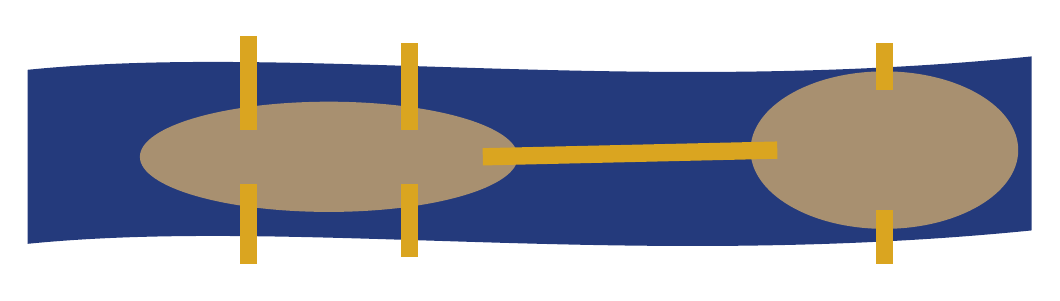
\begin{tikzpicture}[x=0.85mm, y=0.85mm]\koenigsberg;\end{tikzpicture}
\end{frame}

\begin{frame}{Königsberg als Graph?}
  \centering\vspace*{4mm}
  \begin{tikzpicture}[x=0.85mm, y=0.85mm]
    \koenigsberg;
    \begin{scope}[visible on=<2->, font=\Large\bfseries, text=textFg]
      \node at (40,50) {A}; \node at (45,27) {B}; \node at (128,28) {C}; \node at (55,4) {D};
    \end{scope}
  \end{tikzpicture}
\end{frame}

\begin{frame}{Königsberger Graph}
  \centering
  \begin{graph}[x=12mm, y=11.5mm]
    \node[vertex] (A) at (0,2) {A}; \node[vertex] (B) at (0,0) {B};
    \node[vertex] (C) at (2.2,0.2) {C}; \node[vertex] (D) at (-0.6,-1.9) {D};
    \path (A) edge[bend left=25] (B) (A) edge[bend right=25] (B) (B) edge[bend left=25] (D) (B) edge[bend right=25] (D)
          (B) edge (C) (A) edge[bend left=30] (C) (D) edge[bend right=30] (C);
  \end{graph}
\end{frame}

\begin{frame}{Pfade}
  \begin{columns}[T,onlytextwidth]
    \begin{column}{0.5\textwidth}
      \begin{itemize}
        \item Ein \term{Pfad} ist eine Folge von Knoten $v_0, v_1, v_2, \dots, v_n$, wobei $v_i$ und $v_{i+1}$
          jeweils durch eine Kante verbunden sein müssen.
        \begin{itemize}
          \item A, B, C \yes
          \item B, A, B, E, F \yes
          \item A, C, B \no
          \item F, H, G, C, D, E \yes
        \end{itemize}
      \end{itemize}
    \end{column}
    \begin{column}{0.48\textwidth}
      \vspace*{6mm}
      \begin{graph}[x=4.6mm, y=4.6mm, vertex/.append style={minimum size=5.5mm, font=\scriptsize\bfseries}]
        \roadnodes{}
        \path (A) edge (B) (A) edge (E) (B) edge (C) (B) edge (E) (C) edge (D) (C) edge (F) (C) edge (G) (D) edge (E)
              (F) edge (E) (F) edge (H) (G) edge (H) (G) edge (K) (H) edge (K) (K) edge (Z) (H) edge (J) (H) edge (I)
              (J) edge (Z) (E) edge (I) (I) edge (Z);
      \end{graph}
    \end{column}
  \end{columns}
\end{frame}

\begin{frame}{Der Königsberger Pfad}
  \begin{concept}[Eulerpfad]
    Ein Pfad, bei welchem jede Kante eines Graphen genau einmal benutzt wird, nennt man \term{Eulerpfad}.
  \end{concept}
  \pause
  \begin{concept}[Eulertour]
    Ein Eulerpfad, der wieder am Ausgangspunkt endet, ist eine \term{Eulertour}.
  \end{concept}
\end{frame}

\begin{frame}{Königsberger Graph}
  \begin{columns}[T,onlytextwidth]
    \begin{column}{0.55\textwidth}
      \begin{itemize}
        \item Hat dieser Graph
        \begin{itemize}
          \item einen Eulerpfad?
          \item eine Eulertour?
        \end{itemize}
        \item Wann ist ein Graph \term{eulersch}?
        \begin{itemize}
          \item Aufgabe 3 lösen!
        \end{itemize}
      \end{itemize}
    \end{column}
    \begin{column}{0.4\textwidth}
      \centering
      \begin{graph}[x=10mm, y=10mm]
        \node[vertex] (A) at (0,2) {A}; \node[vertex] (B) at (0,0) {B};
        \node[vertex] (C) at (2.2,0.2) {C}; \node[vertex] (D) at (-0.6,-1.9) {D};
        \path (A) edge[bend left=25] (B) (A) edge[bend right=25] (B) (B) edge[bend left=25] (D) (B) edge[bend right=25] (D)
              (B) edge (C) (A) edge[bend left=30] (C) (D) edge[bend right=30] (C);
      \end{graph}
    \end{column}
  \end{columns}
\end{frame}

\begin{frame}{Eulersche Regel}
  \begin{concept}[Eulersche Regel]
    Ein zusammenhängender Graph enthält genau dann einen Eulerpfad, wenn zwei oder keiner seiner Knoten
    einen ungeraden Kantengrad haben.
  \end{concept}
  \begin{itemize}
    \item Sind alle Kantengrade gerade, so existiert eine Eulertour.
  \end{itemize}
\end{frame}

\begin{frame}[read={Algorithmus von Fleury}]{Finden einer Eulertour}
  \begin{enumerate}
    \item Wähle einen beliebigen Knoten als aktuellen Knoten.
    \item Wähle eine unmarkierte Kante, welche vom aktuellen Knoten aus wegführt. Wähle zuerst diejenigen,
      die den unmarkierten Teilgraphen zusammenhängend halten.
    \item Markiere die gewählte Kante.
    \item Nimm den Endpunkt der gewählten Kante als aktuellen Knoten.
    \item Falls noch nicht alle Kanten markiert sind, gehe zu 2.
  \end{enumerate}
\end{frame}

\begin{frame}{Fleury in Action}
  \begin{columns}[T,onlytextwidth]
    \begin{column}{0.5\textwidth}
      \begin{itemize}
        \only<1>{\item Wir wählen F als Startknoten.
          \item Wähle danach eine Kante von F aus.
          \begin{itemize}\item z.\,B. F → B\end{itemize}}%
        \only<2>{\item B wird zum aktuellen Knoten (Endpunkt der gewählten Kante).}%
        \only<3>{\item Wähle von B aus die nächste Kante.
          \begin{itemize}\item z.\,B. B → A\end{itemize}}%
        \only<4>{\item Kante A → F darf (noch) nicht gewählt werden, da F sonst abgeschnitten wäre.
          \begin{itemize}\item A → F ist eine \term{Brückenkante}.\end{itemize}}%
        \only<5>{\item Abgekürzt: Wähle z.\,B. C → E → D.
          \item Nun darf Kante D → A (noch) nicht gewählt werden, sonst wären A und F abgeschnitten.}%
        \only<6>{\item Rest markieren:
          \begin{itemize}\item z.\,B. D → C → B → D → A → F\end{itemize}
          \item Fertig: F → B → A → C → E → D → C → B → D → A → F}
      \end{itemize}
    \end{column}
    \begin{column}{0.44\textwidth}
      \centering
      \begin{graph}[x=11mm, y=11mm]
        \node[vertex] (E) at (1.88,3.85) {E};
        \node[vertex] (C) at (0,2.73) {C};   \node[vertex, onslide=<5>{vertex_active}] (D) at (3.7,2.68) {D};
        \node[vertex, onslide=<4>{vertex_active}] (A) at (0,1.15) {A};
        \node[vertex, onslide=<2-3>{vertex_active}] (B) at (3.7,1.08) {B};
        \node[vertex, onslide=<1>{vertex_active}] (F) at (1.88,0) {F};
        \path (F) edge[onslide=<1->{chosen}] (B) (B) edge[onslide=<3->{chosen}] (A)
              (A) edge[onslide=<5->{chosen}] (C) (C) edge[onslide=<5->{chosen}] (E) (E) edge[onslide=<5->{chosen}] (D)
              (D) edge[onslide=<6->{chosen}] (C) (C) edge[onslide=<6->{chosen}] (B) (B) edge[onslide=<6->{chosen}] (D)
              (D) edge[onslide=<5>{removed}, onslide=<6->{chosen}] (A) (A) edge[onslide=<4>{removed}, onslide=<6->{chosen}] (F);
      \end{graph}
      \vspace{3mm}\stepdots{6}
    \end{column}
  \end{columns}
\end{frame}

\begin{frame}[doit={Aufgabe 4}]{Ihr seid dran: Staubsaugen!}
  \vfill
  \RTask{4}{Staubsaugen}{Löst Aufgabe 4 im Skript.}
  \vfill
\end{frame}

\begin{frame}{Staubsaugen}
  \begin{itemize}
    \item Fragen / Unklarheiten?
  \end{itemize}
\end{frame}

\begin{frame}[doit={Aufgabe 5}]{Rätsel: Teeren}
  \vfill
  \RTask{5}{Teeren}{Löst Aufgabe 5 im Skript.}
  \vfill
\end{frame}

\section{Spannbäume}
\begin{frame}{(Spannende) Bäume}
  \begin{concept}[Baum]
    Ein \term{Baum} ist ein zusammenhängender Graph, welcher keinen Kreis enthält.
  \end{concept}
  \centering
  \begin{graph}[x=8.5mm, y=7.5mm]
    \begin{scope}
      \node[vertex] (E) at (1.5,2) {E}; \node[vertex] (C) at (0,1.2) {C}; \node[vertex] (D) at (3,1.2) {D};
      \node[vertex] (A) at (0,0) {A}; \node[vertex] (F) at (1.5,-0.5) {F}; \node[vertex] (B) at (3,0) {B};
      \path (E) edge (C) (E) edge (D) (C) edge (A) (A) edge (F) (D) edge (B);
      \node[font=\Large, text=termColor] at (4,-0.5) {\yes};
    \end{scope}
    \begin{scope}[xshift=70mm]
      \node[vertex] (E) at (1.5,2) {E}; \node[vertex] (C) at (0,1.2) {C}; \node[vertex] (D) at (3,1.2) {D};
      \node[vertex] (A) at (0,0) {A}; \node[vertex] (F) at (1.5,-0.5) {F}; \node[vertex] (B) at (3,0) {B};
      \path (E) edge (C) (E) edge (D) (C) edge (A) (A) edge (F) (D) edge (B) (F) edge (B);
      \node[font=\Large, text=termColor] at (4,-0.5) {\no};
    \end{scope}
  \end{graph}
\end{frame}

\begin{frame}{(Spannende) Bäume}
  \begin{concept}[Spannbaum]
    Ein \term{Spannbaum} eines Graphen $G$ ist ein Baum, der alle Knoten von $G$ enthält.
  \end{concept}
  \centering
  \begin{graph}[x=8mm, y=8mm, vertex/.append style={minimum size=6.5mm, font=\footnotesize\bfseries}]
    \roadnodes{}
    \path (A) edge[chosen] (B) (A) edge (E) (B) edge[chosen] (C) (B) edge (E) (C) edge[chosen] (D) (C) edge (F) (C) edge (G)
          (D) edge[chosen] (E) (F) edge[chosen] (E) (F) edge[chosen] (H) (G) edge[chosen] (H) (G) edge (K) (H) edge[chosen] (K)
          (K) edge (Z) (H) edge[chosen] (J) (H) edge (I) (J) edge[chosen] (Z) (E) edge (I) (I) edge[chosen] (Z);
  \end{graph}
\end{frame}

\begin{frame}{(Spannende) Bäume}
  \begin{concept}[Minimaler Spannbaum]
    Ein \term{minimaler Spannbaum} ist ein Spannbaum, bei dem die Summe der Kantengewichte minimal ist.
  \end{concept}
\end{frame}

\begin{frame}{Algorithmus von Kruskal}
  \begin{itemize}
    \item Wähle die billigste Kante und markiere sie.
    \item Betrachte die restlichen Kanten in aufsteigender Reihenfolge. Für jede Kante:
    \begin{itemize}
      \item Falls die neue Kante mit den markierten Kanten zusammen keinen Kreis bildet, markiere sie.
        (Sie wird Teil des Spannbaums.)
      \item Ansonsten ist die Kante nicht Teil des Spannbaums.
      \item Sobald alle Knoten erschlossen sind, kannst du abbrechen.
    \end{itemize}
    \item Der Spannbaum besteht aus den markierten Kanten.
  \end{itemize}
\end{frame}

\begin{frame}{Greedy}
  \begin{itemize}
    \item Kruskal ist ein Beispiel eines \term{Greedy-Algorithmus}.
  \end{itemize}
\end{frame}

\begin{frame}{Kruskal in Action}
  \begin{columns}[T,onlytextwidth]
    \begin{column}{0.5\textwidth}
      \begin{itemize}
        \item<2-> \only<2>{Wähle die günstigste Kante.}\only<3->{Wähle die nächstgünstigste, die keinen Kreis bildet.}%
        \only<4>{\begin{itemize}
            \item A → E würde einen Kreis bilden.
            \item Deshalb wählen wir A → B (oder B → D).
          \end{itemize}}%
        \only<5>{\item Finito!
          \begin{itemize}\item Der Spannbaum hat ein Totalgewicht von 15.\end{itemize}}
      \end{itemize}
    \end{column}
    \begin{column}{0.44\textwidth}
      \centering
      \begin{graph}[x=13mm, y=13mm]
        \node[vertex] (E) at (1.7,2.5) {E}; \node[vertex] (C) at (0,1.5) {C}; \node[vertex] (D) at (3.33,1.4) {D};
        \node[vertex] (A) at (0.83,0.15) {A}; \node[vertex] (B) at (3.33,0) {B};
        \path (C) edge["3", onslide=<3->{chosen}] (E) (E) edge["8"] (D) (C) edge["10"] (D)
              (A) edge["4", onslide=<4->{removed}] (E) (A) edge["6"] (D) (C) edge["2", onslide=<2->{chosen}] (A)
              (D) edge["5", onslide=<5->{chosen}] (B) (A) edge["5", onslide=<4->{chosen}] (B);
      \end{graph}
      \vspace{3mm}\stepdots{5}
    \end{column}
  \end{columns}
\end{frame}

\end{document}
